\documentclass[11pt]{article}
\usepackage{listings, ../listings-rust/listings-rust}
\usepackage{xcolor}
\usepackage{algorithm}
\usepackage[noend]{algpseudocode} % pseudocode
\usepackage{amsmath,amsthm,amssymb}
\usepackage {tikz}
\usetikzlibrary{automata, positioning}
\definecolor{codegreen}{rgb}{0,0.6,0}
\definecolor{codegray}{rgb}{0.5,0.5,0.5}
\definecolor{codepurple}{rgb}{0.58,0,0.82}
\definecolor{backcolour}{rgb}{0.95,0.95,0.92}
\lstset{
    language=Python,
    keepspaces=true,
    numbers=left,
    backgroundcolor=\color{backcolour},
    commentstyle=\color{codegreen},
    basicstyle=\ttfamily,
    otherkeywords={self,True,False,yield},
    keywordstyle=\ttfamily\color{blue!90!black},
    %basicstyle=\footnotesize,
    keywords=[3]{ttk},
    keywordstyle={[2]\ttfamily\color{orange!80!orange}},
    keywordstyle={[3]\ttfamily\color{red!80!orange}},
    emph={MyClass,__init__},
    emphstyle=\ttfamily\color{red!80!black},
    stringstyle=\color{green!80!black},
    showstringspaces=false
}
\usepackage{enumerate}
\usepackage{fullpage,amsmath,amssymb,graphicx}
\usepackage[colorlinks=true,citecolor=blue,linkcolor=blue]{hyperref} % for href links, and also makes \ref and \eqref clickable in the PDF
\newcommand{\QuasiP}{\mathsf{QuasiP}}
\newcommand{\TIME}{\mathsf{TIME}}
\newcommand{\N}{\mathbb{N}}
\newcommand{\Z}{\mathbb{Z}}
\renewcommand{\P}{\mathsf{P}}
\newcommand{\NP}{\mathsf{NP}}
\newcommand{\poly}{\mathrm{poly}}
\newcommand{\SAT}{\textsc{Sat}}
\newcommand{\sat}{\SAT}
\newcommand{\dnfsat}{\textsc{DNF-\sat}}
\newcommand{\cnfsat}{\textsc{CNF-\sat}}
\newcommand{\pmat}{\textsc{Perfect-Matching}}
\newcommand{\iset}{\textsc{Independent-Set}}
\newcommand{\cpc}{\textsc{Cellphone-Capacity}}
\usepackage{fancyhdr}
\fancypagestyle{firststyle}
{
   \fancyhf{}
   \fancyhead[C]{Copyright \copyright\ \today, David Doty}
}
\title{Homework 3 -- ECS 220, Winter 2020}
\date{}
\begin{document}
\maketitle
\thispagestyle{firststyle}
\vspace{-2.0cm}

\section*{Really independent sets}
    \begin{quote}
    Given a graph $G = (V,E)$, say that a subset $S \subseteq V$ is \emph{really independent} if there are no $u,v \in S$ that are two or fewer steps apart in the graph---that is, if for all $u,v \in S$, the length of the shortest path
    between $u$ and $v$ is at least 3.
    The problem \textsc{ReallyIndependentSet} takes a graph $G$ and an integer $k$ as input, and asks if $G$ has a really independent set of size $k$ or more.
    Prove that \textsc{ReallyIndependentSet} is $\NP$-complete.
    \end{quote}

We are going to show that \textsc{ReallyIndependentSet} is at least as hard as \textsc{IndependentSet}, i.e. we are going to reduce \textsc{IndependentSet} to \textsc{ReallyIndependentSet}.

Given any graph $G_3 = (V_3, E_3)$, we are going to do the following changes to make $G_2 = (V_2, E_2)$:

$$V_2 = V_3$$
$$E_2 = E_3 \cup \{(u, v) | u, t, v \in V, (u, t), (t, v) \in E\}$$

Explained in English: We find 3 nodes connected with 2 edges and link them as a triangle.

\begin{center}
	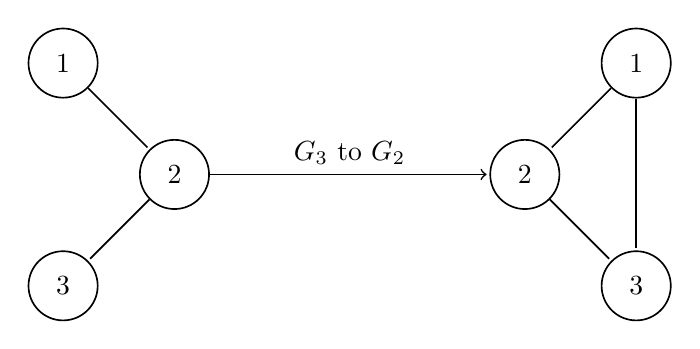
\begin{tikzpicture}[shorten >=1pt,node distance=2cm,on grid,auto, semithick]
		\node[state]		 	(b)	                     		{2};
        \node[state] 			(a) 	[above left=of b]		{1};
        \node[state]			(c)		[below left=of b]		{3};

		\node[state]		 	(bp)	[right=of b, right=4cm] 		    {2};
		\node[state] 			(ap) 	[above right=of bp]		{1};
        \node[state]			(cp)	[below right=of bp]		{3};
		\path[-]
			(a)	    edge	node	{}	(b)
			(b)		edge	node	{}	(c)
			(ap)	edge	node	{}	(bp)
            (bp)	edge	node	{}	(cp)
            (ap)	edge	node	{}	(cp)
            ;
        \path[->]
            (b)		edge	node	{$G_3$ to $G_2$}	(bp)
            ;
    \end{tikzpicture}
\end{center}

\textbf{Claim: The reduction happens in polynomial time.}
\begin{proof}
    Enumerate all possible 3-node combinations took $O(|V|^3)$ time.
\end{proof}

Let's denote the Independent Set being $I$, $I_3$ begin \textsc{ReallyIndependentSet}, $I_2$ being \textsc{IndependentSet}.

\textbf{Claim: If $G_3$ has $|I_3| = k$, it's derived $G_2$ has $|I_2| = k$ and $I_3 = I_2$}.
\begin{proof}

    $\forall u, v \in I_3$, $\texttt{distance}(G_3, u, v) \ge 3$, suppose the shortest path being $(u, t_1), (t_1, t_2) \cdots (t_c, v)$, we know $c \ge 2$ for the distance's sake. Therefore according to our reduction, $(u, t_2), (t_{c-1}, v) \in E_2, \forall i, s.t. i+2 \le c \rightarrow (t_i, t_{i+2}) \in E_2$.
    
    Given this relation, we are safe to conclude that in $G_2$, $\texttt{distance}(G_2, u, v) \ge 2$.

    Therefore all nodes in $I_3$ consists of an indenpent set in $G_2$, i.e. $I_3 = I_2$.
\end{proof}

\textbf{Claim: For $G_3$ and derived $G_2$,  $\forall I_3, |I_3| < k \rightarrow \forall I_2, |I_2| < k$}

Hint: This is to proof that if there is no \textsc{ReallyIndependentSet} of size $k$, there is no \textsc{IndependentSet} of size $k$ either.

\begin{proof}
    Let's proof by contradiction.

    Suppose $\exists I_2, |I_2| = k$, $\exists u, v \in I_2, \texttt{distance}(G_3, u, v) = 2$.
    (If $\forall u, v, \texttt{distance} \ge 3$, then $I_3 = I_2$ and we found our \textsc{ReallyIndependentSet}, if $ \texttt{distance}(G_3, u, v) = \texttt{distance}(G_3, u, v) = 1$, then it's not an \textsc{IndependentSet} for $G_2$).

    Since $\texttt{distance}(G_3, u, v) = 2$, without loss of generality let's denote the node in the middle $t$.
    According to our reduction, $(u, t), (t, v) \in E_2 \rightarrow \texttt{distance}(G_2, u, v) = 1$, again, $I_2$ would not be an \textsc{IndependentSet} by then.
\end{proof}

With the properties proved above, we can finalize our reduction algorithm to solve \textsc{IndependentSet}:

\begin{enumerate}
    \item Given $G_3$, convert it to $G_2$.
    \item The answer to \textsc{IndependentSet} of $G_2$ is the same as \textsc{ReallyIndependentSet} in $G_3$.
\end{enumerate}

\end{document}
